\documentclass[preprint,authoryear,12pt]{elsarticle}

\usepackage{graphicx}
\usepackage{url}		% Display web addresses nicely
\usepackage{amsfonts,amssymb,amsbsy,amsmath,amscd}

\RequirePackage{latexsym,ifthen,theorem,booktabs}
\RequirePackage{amsfonts,amssymb,amsbsy,amsmath,amscd}
\usepackage{verbatim}
\biboptions{sort}

% Shortcuts / styling
\newcommand{\secref}[1]{Section~\ref{#1}}
\newcommand{\code}[1]{\texttt{#1}}
\newcommand{\Matlab}{{\sc Matlab}\textsuperscript{\textregistered}}
% A value with units
\newcommand{\vu}[2]{\ensuremath{#1\,\mathrm{#2}}}

\newcommand{\ud}{\mathrm{d}}
\newcommand{\dt}{\ud t}
\newcommand{\dd}[2]{{\ud #1}/{\ud #2}}

% Authors' notes
\usepackage{color}
%\newcommand{\authornote}[2]{{\bf\color{red} [#1: #2]}}
\newcommand{\authornote}[2]{{\bf [#1: #2]}}
\newcommand{\jc}[1]{\authornote{Jon}{#1}}
\newcommand{\gary}[1]{\authornote{Gary}{#1}}
\newcommand{\steve}[1]{\authornote{Steve}{#1}}

%\newcommand{\changed}[1]{\textcolor{cyan}{#1}}
\newcommand{\changed}[1]{#1}

\graphicspath{{images/}}

% Title page info
\journal{Progress in Biophysics and Molecular Biology}
\begin{document}

\appendix

\makeatletter
\renewcommand{\thefigure}{S\@arabic\c@figure}
\renewcommand{\thetable}{S\@arabic\c@table}
\makeatother
\setcounter{figure}{0}
\setcounter{table}{0}

%%%%%%%%%%%%%%%%%%%%%%%%%%%%%%%%%%%%%%%%%%%%%%%%%%%%%%%%%%%%%%%%%%%%%%
\section{Details of S1-S2 Protocol Post-processing}
\label{supp:case-study-details}
%%%%%%%%%%%%%%%%%%%%%%%%%%%%%%%%%%%%%%%%%%%%%%%%%%%%%%%%%%%%%%%%%%%%%%

Within the main text there was space to give only a high-level description of the S1-S2 protocol used as a case study (see Section~2.5.1).
In this section we give further details of how the various post-processing functions used were implemented, building on the basic operations provided by the language.


The actual post-processing definition for this protocol is very short, consisting of just 5 steps.
Firstly the raw APD and DI values are computed for all time-courses, using the \code{apd} function, which encapsulates the bulk of the complexity for this protocol.
Secondly, the APD and DI values of interest are extracted using a \code{view} operation---for each S2 interval, we take the first DI and the second APD.
Finally, we filter the results to remove entries corresponding to an S2 interval which yielded a DI less than \vu{19}{ms}, for reasons described in the main text.
This is achieved by a combination of \code{map} (to test where the DI value is greater than \vu{19}{ms}), \code{find} (to locate the corresponding indices), and \code{index} (to index the APD and DI arrays).
This conciseness is achievable due to the use of complex functions, which could be provided in a standard library.
These include the following functions.


\begin{description}
\item[apd]
  This is the main post-processing function used in the S1-S2 protocol, which makes use of both the basic operations in the language, and the other compound functions described below.
  It takes 3 compulsory inputs: arrays representing $V$ and $t$, and the percentage APD to compute.
  There are also 3 optional inputs.
  The first is the dimension over which time varies, which defaults to the last dimension, since the time-course simulation is typically the innermost in a nested simulation.
  The others are used to fine tune the algorithm, and will be described where they are used.
  The algorithm itself consists of several steps.
  \begin{enumerate}
  \item
    The \code{gradient} function is used to compute the gradient $\dd{V}{t}$ of $V$ with respect to $t$.
  \item
    Local maxima of $\dd{V}{t}$ are located using a \code{window} operation, with the window size given by an optional parameter defaulting to 50.
    This must be set large enough that only one such maximum is found for each AP upstroke.
    The maxima are filtered so that only those above a threshold (another optional parameter, defaulting to \vu{10}{mV}) are retained, to remove local maxima that occur away from an upstroke.
  \item
    The indices of these maxima are found using \code{find}, and used to \code{index} the $t$ array to yield an array of upstroke times.
    This array is padded with a fake upstroke time, in case not all simulations produced the same number of APs.
    The extent of the time dimension then gives the maximum number of APs in any time-course simulation.
  \item
    The algorithm now operates on extended arrays containing one more dimension than the inputs.
    Suppose $V$ and $t$ both have $\mathit{ND}$ dimensions, where $\mathit{ND} \geq 1$.
    In our example protocol, $\mathit{ND}=2$.
    Let $N$ represent the sizes of the first $\mathit{ND}-1$ dimensions, which come from the outer loops in a nested simulation.
    Let $T$ be the size of the last (time) dimension, and let $A$ be the maximum number of APs.
    Extended arrays then have shape $N$x$A$x$T$.
    Each time-course simulation is replicated along the new dimension (using array creation functionality), and subsequent operations focus on a different region of the time-course for each AP, using the maximum upstroke times to locate these regions.
  \item
    The peak voltage in each AP is determined by taking local maxima of the $V$ array (with a window size of 1), then \code{find}ing locations where the extended $V$ array is equal to these peaks and the extended $t$ array is greater than the maximum upstroke times array.
    The extended $V$ array is then \code{index}ed and the first occurrence taken for each AP using a \code{view} operation.
    The resting potential could be determined in a similar fashion, or we can take a global minimum.
  \item
    Given the peak and resting potentials, and the input percentage value, a \code{map} yields the desired repolarisation potentials.
  \item
    Next, linear interpolation (defined by the \code{interp} function) is used twice to locate the first times before and after each peak where the repolarisation potential is reached, and these times are taken as the start and end of each AP; the difference between them is the APD, and is obtained by a \code{map}.
  \item
    Finally, the DI values are obtained by again taking the element-wise difference between two arrays using \code{map}: the first array containing the intervals between AP starts (computed using \code{diff}), and the second being a \code{view} of the APDs, with the last APD removed for each run (i.e.\ S2 interval in our case).
  \end{enumerate}

  Besides the basic functionality built-in to the post-processing language, APD calculation thus makes use of the additional functions defined below.
  These are \code{diff}, \code{gradient}, \code{maximum} (and \code{minimum}), \code{window}, and \code{interp}.

\item[diff]
  The \code{diff} function computes the difference between successive elements in an array along a given dimension.
  This requires a \code{map} of the minus operator onto two \code{view}s of the input array: the first of which omits the first entry, and the second of which omits the last, along the desired dimension.

\item[gradient]
  This function computes gradients, given $x$ and $y$ inputs.
  By utilising the \code{diff} function applied to each input, it only requires one additional \code{map} of the division operator to compute ``change in $y$ over change in $x$.''

\item[maximum]
  By folding the operator \code{max} that computes the maximum of two values along a desired dimension, the maximum values in the input array along that dimension can be determined.
  The \code{minimum} function is defined equivalently.

\item[window]
  The \code{window} function enables the effect of allowing post-processing operations, which operate on whole arrays, to be applied at a local level on a sliding window over an input array.
  For example, rather than finding a global maximum, one can use \code{window} and \code{maximum} to compute an array each entry of which is the maximum within a small window centred on the equivalent entry of the input.
  This is done by creating an intermediate array using the \code{window} function which has one more dimension than the input.
  The window around an entry then appears along the new dimension, and the maximum may be taken along this dimension also.
  The definition of \code{window} uses only the \code{shift} function (defined below) along with basic array creation functionality.

\item[shift]
  This function shifts an array a given distance along the specified dimension.
  The result is an array of the same size as the input, padded with the initial entry at the end being shifted away from.
  It is used to compute the sub-arrays of a \code{window} operation.

\item[interp]
  This function performs linear interpolation, either forwards or backwards along a specified dimension.
  It takes four compulsory inputs: the $x$ and $y$ arrays, target $y$ values $y_t$, and an array of starting positions $x_s$ along the $x$ axes, and interpolates $x$ to determine the first value either before or after the start point for which $y$ equals the target.
  If the inputs have more than one dimension, this function thus performs multiple interpolations at once.
  There are several steps.
  \begin{enumerate}
  \item
    The first step is to find indexes $i$ into $y$ such that $x[i] \geq s$, and, if $y$ at $x_s$ is greater than $y_t$, $y[i] \leq y_t$, otherwise $y[i] \geq y_t$.
    This in itself is done in several steps.
    \begin{enumerate}
    \item
      First, array creation functionality is used to replicate $S$ and $T$ to the size of $x$ and $y$.
      Then \code{map}, \code{find}, and \code{index} are used to find the values $y_s$ of $y$ where $x = s$.
    \item
      Another \code{map} creates an array containing $1$ only where the second part of the predicate holds, i.e.\ where if $y_s > y_t$, then $y \leq y_t$ holds, or if $y_s < y_t$ then $y \geq y_t$ holds.
    \item
      A further \code{map} creates an array containing $1$ only where the above array is $1$ and $x$ values are suitable, i.e. where $x \geq x_s$ if we are searching forwards, or $x \leq x_s$ if searching backwards.
    \item
      Finally, \code{find} on this array yields the desired indices.
    \end{enumerate}
  \item
    For each interpolation being calculated, the result should be $x[i]$ if $i=0$, or $x[i-1] + (x[i]-x[i-1])(y_t-y[i-1])/(y[i]-y[i-1])$ otherwise.
    (If searching backwards, the special case is when $i$ is the last index, and the expression is $x[i] + (x[i+1]-x[i])(y_t-y[i])/(y[i+1]-y[i])$.)
    In order to compute all interpolations being asked for, an array containing these values must be constructed using array operations.
    The final step will be to index it.
    Firstly, we compute the \code{gradient} $g$ of $x$ over $y$, which when indexed will yield $(x[i]-x[i-1])/(y[i]-y[i-1])$.
    Array creation functionality is used to concatenate this with a zero array to handle the $i=0$ case, giving a result the same size as $x$ etc.
  \item
    Next \code{map} is used to compute $y_t - y$, which is shifted one entry to the right if searching forwards.
    Call this $\tilde{y}$.
    A similarly shifted copy of $x$, $\tilde{x}$, is also calculated.
  \item
    A \code{map} is then used to calculate $\tilde{x} + \tilde{y} g$, and this is indexed with the array from the first step.
  \item
    Finally, a \code{view} is used to select the first or last entries, depending on the direction of search.
  \end{enumerate}

\end{description}


%%%%%%%%%%%%%%%%%%%%%%%%%%%%%%%%%%%%%%%%%%%%%%%%%%%%%%%%%%%%%%%%%%%%%%
\section{Supplementary Figures}
\label{supp:figures}
%%%%%%%%%%%%%%%%%%%%%%%%%%%%%%%%%%%%%%%%%%%%%%%%%%%%%%%%%%%%%%%%%%%%%%

In Figures~\ref{fig:S1S2_Curves:rest1} and \ref{fig:S1S2_Curves:rest2} we display the results of the S1-S2 protocol for the models which were not shown in the main text in Figures~4 and 5.

\begin{figure}
\begin{center}
%
% Commented out ones have mental DADs which are throwing the calculations at present
%
\includegraphics[width=0.32\linewidth]{aslanidi_Purkinje_model_2009_s1s2_curve}
\includegraphics[width=0.32\linewidth]{beeler_reuter_model_1977_s1s2_curve}
\includegraphics[width=0.32\linewidth]{bondarenko_szigeti_bett_kim_rasmusson_2004_apical_s1s2_curve}
\includegraphics[width=0.32\linewidth]{corrias_purkinje_2011_s1s2_curve}
\includegraphics[width=0.32\linewidth]{courtemanche_ramirez_nattel_1998_s1s2_curve}
\includegraphics[width=0.32\linewidth]{earm_noble_model_1990_s1s2_curve}
\includegraphics[width=0.32\linewidth]{espinosa_model_1998_normal_s1s2_curve}
\includegraphics[width=0.32\linewidth]{faber_rudy_2000_s1s2_curve}
\includegraphics[width=0.32\linewidth]{hilgemann_noble_model_1987_s1s2_curve}
\includegraphics[width=0.32\linewidth]{iribe_model_2006_s1s2_curve}
\includegraphics[width=0.32\linewidth]{iyer_2004_s1s2_curve}
%\includegraphics[width=0.32\linewidth]{jafri_rice_winslow_model_1998_s1s2_curve}
\includegraphics[width=0.32\linewidth]{lindblad_model_1996_s1s2_curve}
\caption{S1-S2 restitution curves for models (S1$ = 1000$ms).}
\label{fig:S1S2_Curves:rest1}
\end{center}
\end{figure}

\begin{figure}
\begin{center}
\includegraphics[width=0.32\linewidth]{luo_rudy_1991_s1s2_curve}
\includegraphics[width=0.32\linewidth]{mahajan_shiferaw_2008_s1s2_curve}
%\includegraphics[width=0.32\linewidth]{maleckar_model_2009_s1s2_curve}
\includegraphics[width=0.32\linewidth]{matsuoka_model_2003_s1s2_curve}
\includegraphics[width=0.32\linewidth]{noble_model_1991_s1s2_curve}
%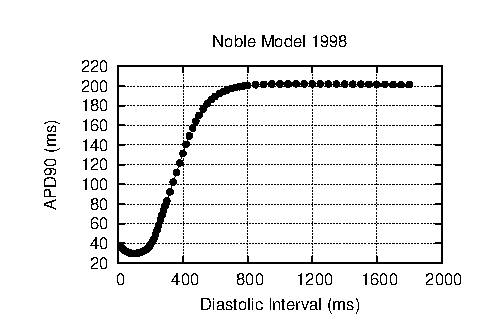
\includegraphics[width=0.32\linewidth]{noble_model_1998_s1s2_curve}
%\includegraphics[width=0.24\linewidth]{nygren_atrial_model_1998_s1s2_curve}
\includegraphics[width=0.32\linewidth]{pandit_clark_giles_demir_2001_epicardial_cell_s1s2_curve}
\includegraphics[width=0.32\linewidth]{pasek_simurda_orchard_christe_2008_s1s2_curve}
\includegraphics[width=0.32\linewidth]{sakmann_model_2000_epi_s1s2_curve}
\includegraphics[width=0.32\linewidth]{shannon_wang_puglisi_weber_bers_2004_s1s2_curve}
\includegraphics[width=0.32\linewidth]{ten_tusscher_model_2004_epi_s1s2_curve}
\caption{S1-S2 restitution curves for a large number of models (S1$ = 1000$ms).}
\label{fig:S1S2_Curves:rest2}
\end{center}
\end{figure}

In Figures~\ref{fig:ICaL_IV_curves:rest1} and \ref{fig:ICaL_IV_curves:rest2} we present the L-type calcium channel IV curves for the remaining models that were not shown in Figure~6 of the main text, apart from Beeler and Reuter (1977) (which does not feature an L-type calcium current). Only one curve is shown for Luo and Rudy (1991) as it does not feature extracellular calcium.



\begin{figure}
\begin{center}
\includegraphics[width=0.32\linewidth]{earm_noble_model_1990_ICaL_IV_curve}
\includegraphics[width=0.32\linewidth]{espinosa_model_1998_normal_ICaL_IV_curve}
\includegraphics[width=0.32\linewidth]{faber_rudy_2000_ICaL_IV_curve}
\includegraphics[width=0.32\linewidth]{fink_noble_giles_model_2008_ICaL_IV_curve}
\includegraphics[width=0.32\linewidth]{hilgemann_noble_model_1987_ICaL_IV_curve}
\includegraphics[width=0.32\linewidth]{hund_rudy_2004_ICaL_IV_curve}
\includegraphics[width=0.32\linewidth]{iribe_model_2006_ICaL_IV_curve}
\includegraphics[width=0.32\linewidth]{iyer_model_2007_ICaL_IV_curve}
\caption{I$_\textrm{CaL}$ IV curves for the models, generated by recording the largest L-type calcium current resulting from a voltage clamp from a holding potential of $-50$mV to the test voltage plotted. Solid lines 50\%, dashed lines 100\%, dotted lines 150\% of model's default extracellular calcium concentration.}
\label{fig:ICaL_IV_curves:rest1}
\end{center}
\end{figure}

\begin{figure}
\begin{center}
%\includegraphics[width=0.32\linewidth]{li_mouse_2010_ICaL_IV_curve}
\includegraphics[width=0.32\linewidth]{lindblad_model_1996_ICaL_IV_curve}
\includegraphics[width=0.32\linewidth]{luo_rudy_1991_ICaL_IV_curve}
\includegraphics[width=0.32\linewidth]{matsuoka_model_2003_ICaL_IV_curve}
\includegraphics[width=0.32\linewidth]{noble_model_1991_ICaL_IV_curve}
\includegraphics[width=0.32\linewidth]{pandit_clark_giles_demir_2001_endocardial_cell_ICaL_IV_curve}
\includegraphics[width=0.32\linewidth]{pasek_simurda_orchard_christe_2008_ICaL_IV_curve}
\includegraphics[width=0.32\linewidth]{priebe_beuckelmann_1998_ICaL_IV_curve}
\includegraphics[width=0.32\linewidth]{sakmann_model_2000_epi_ICaL_IV_curve}
\caption{I$_\textrm{CaL}$ IV curves for the models, generated by recording the largest L-type calcium current resulting from a voltage clamp from a holding potential of $-50$mV to the test voltage plotted. Solid lines 50\%, dashed lines 100\%, dotted lines 150\% of model's default extracellular calcium concentration.}
\label{fig:ICaL_IV_curves:rest2}
\end{center}
\end{figure}

\end{document}
